% Don't touch this %%%%%%%%%%%%%%%%%%%%%%%%%%%%%%%%%%%%%%%%%%%
\documentclass[11pt]{article}
\usepackage{fullpage}
\usepackage[left=1in,top=1in,right=1in,bottom=1in,headheight=3ex,headsep=3ex]{geometry}
\usepackage{graphicx}
\usepackage{float}

\newcommand{\blankline}{\quad\pagebreak[2]}
\newcommand{\comment}[1]{}

\usepackage{setspace}
\usepackage{multicol}
%\usepackage{indentfirst}
\usepackage{fancyhdr,lastpage}
\usepackage{url}
\pagestyle{fancy}
\usepackage{hyperref}
\usepackage{lastpage}
\usepackage{amsmath}
\usepackage{layout}
\usepackage{enumitem}

\usepackage{array}
\usepackage{booktabs}
\graphicspath{{graphics/}{graphics/movies/}{graphics/images/}}

\lhead{}
\chead{}
\rhead{\footnotesize MATH-151 Mathematical Algorithms in Matlab - Fall 2023}

\lfoot{}
\cfoot{\small \thepage/\pageref*{LastPage}}
\rfoot{}

\usepackage{array, xcolor}
\usepackage{color,hyperref}
\hypersetup{colorlinks,breaklinks,linkcolor=blue,urlcolor=blue,anchorcolor=blue,citecolor=black}

%%%%%%%%%%%%%%%%%%%%%%%%%%%%%%%%%%%%%%%%%%%%%%%%%%%%%
%%%%%%%%%%%%%%%%%%%%%%%%%%%%%%%%%%%%%%%%%%%%%%%%%%%%%
%%%%%%%%%%%%%%%%%%%%%%%%%%%%%%%%%%%%%%%%%%%%%%%%%%%%%

\begin{document}
	
	\begin{center}
		\Large{\textbf{MATH-151 Final Lab Journal}}\\
	\end{center}
	\noindent\makebox[\linewidth]{\rule{\textwidth}{0.4pt}}
	%%%%%%%%%%%%%%%%%%%%%%%%%%%%%%%%%%%%%%%%%%%%%%%%%%%%%
	%%%%%%%%%%%%%%%%%%%%%%%%%%%%%%%%%%%%%%%%%%%%%%%%%%%%%	
	\section*{Task 1: Going on Cruise Control}
	\begin{enumerate}[label=\alph*)]
		\item We have found our optimal P gain to be about 1.45, see plot below. We know this will minimize settling time because it is the zero of the derivative as it transitions from negative values (setting times decreasing) to positive values (settling times increasing). \\
		\begin{center}
			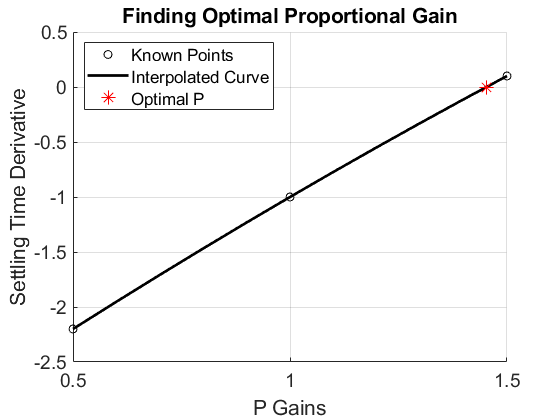
\includegraphics[width = 5cm]{Part_a_Minimizer.png}
		\end{center}
		
		\item We can see in this plot that the car attempts to accelerate from 40 mph to 50 mph very rapidly. There is a steep increase in speed, however it still does not reach 50mph in the end.. However, our first concern should be the safety of our drivers and tone down that acceleration a bit.\\
			\begin{center}
				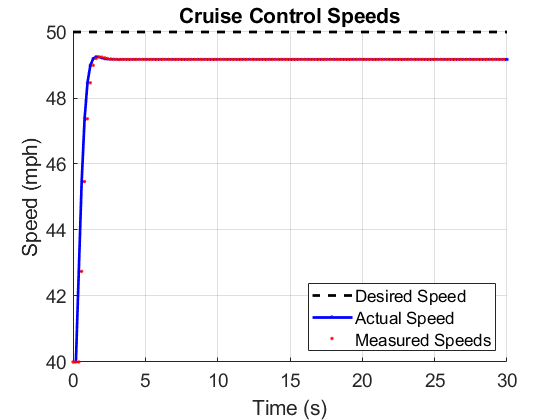
\includegraphics[width = 5cm]{Part_b.png}
			\end{center}
		
		\item Now we see our initial acceleration is slower, that is showing up as a less steep slope at the beginning as the vehicle tries to come up to speed. But we still don't get to 50 mph.\\
			\begin{center}
				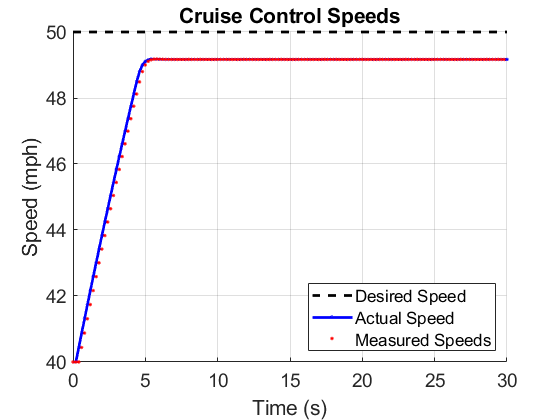
\includegraphics[width = 5cm]{Part_c.png}
			\end{center} 
		\item The integral has helped our controller give the extra push we needed to actually reach 50mph, but we get into a vicious cycle where it overshoots the desired speed and then overcompensates by slowing down, which it overshoots and overcompensates by accelerating too much. We'll need to smooth that out.\\
			\begin{center}
				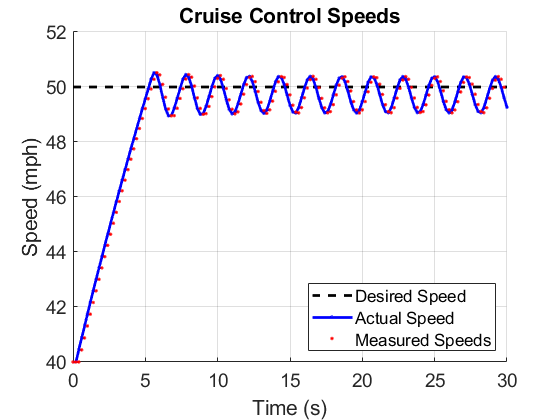
\includegraphics[width = 5cm]{Part_d.png}
			\end{center}
		\item The derivative gain helped us out by leveling out the curve and counteracting some of the integral overcompensations we saw from the integral gain. We now have a smooth ride that is close to our commanded speed even though it ultimately doesn't settle in at that speed.\\
			\begin{center}
				\includegraphics[width = 5cm]{Part_e.png}
			\end{center}
		\item In the end, I think this seems like a somewhat reasonable controller. It doesn't quite settle in at the speed that we'd want so I think adjusting out proportional gain would be the most helpful for this to help us overcome the drag forces, but there are many things we could do to address it. 
	\end{enumerate}
	\begin{center}
		\vfill
		\textit{Thanks everyone! I had fun!}
	\end{center}
\end{document}